%%% Document Author: J Moss
%%% Parts in LaTeX: Nicholas Dart
%%% Other Content: See authors list
%%% Document Last edit: 28.10.2014

\documentclass[11pt, article]{article}
\usepackage{a4wide}
\usepackage[english]{babel}
\usepackage{graphicx}
\usepackage{tabu}
\usepackage{textcomp}
\usepackage{fancyhdr}
\usepackage{lastpage}
\usepackage{titlesec}
\usepackage{lscape}
\usepackage{longtable}
\usepackage{color}
\usepackage{listings}

\definecolor{mygreen}{rgb}{0,0.6,0}
\definecolor{mygray}{rgb}{0.5,0.5,0.5}
\definecolor{mymauve}{rgb}{0.58,0,0.82}

\lstset{ % Syntax highliughting for java
    backgroundcolor=\color{white},   % choose the background color; you must add \usepackage{color} or \usepackage{xcolor}
    basicstyle=\footnotesize,        % the size of the fonts that are used for the code
    breakatwhitespace=false,         % sets if automatic breaks should only happen at whitespace
    breaklines=true,                 % sets automatic line breaking
    captionpos=b,                    % sets the caption-position to bottom
    commentstyle=\color{mygreen},    % comment style
    deletekeywords={...},            % if you want to delete keywords from the given language
    escapeinside={\%*}{*)},          % if you want to add LaTeX within your code
    extendedchars=true,              % lets you use non-ASCII characters; for 8-bits encodings only, does not work with UTF-8
    frame=none,                    % adds a frame around the code
    keepspaces=true,                 % keeps spaces in text, useful for keeping indentation of code (possibly needs columns=flexible)
    keywordstyle=\color{blue},       % keyword style
    language=Octave,                 % the language of the code
    morekeywords={*,...},            % if you want to add more keywords to the set
    numbers=left,                    % where to put the line-numbers; possible values are (none, left, right)
    numbersep=5pt,                   % how far the line-numbers are from the code
    numberstyle=\tiny\color{mygray}, % the style that is used for the line-numbers
    rulecolor=\color{black},         % if not set, the frame-color may be changed on line-breaks within not-black text (e.g. comments (green here))
    showspaces=false,                % show spaces everywhere adding particular underscores; it overrides 'showstringspaces'
    showstringspaces=false,          % underline spaces within strings only
    showtabs=false,                  % show tabs within strings adding particular underscores
    stepnumber=5,                    % the step between two line-numbers. If it's 1, each line will be numbered
    stringstyle=\color{mymauve},     % string literal style
    tabsize=4,                       % sets default tabsize to 2 spaces
    title=\lstname                   % show the filename of files included with \lstinputlisting; also try caption instead of title
}

%%%%%%
%% Variables for version and release status
%% useage: \version
%%%%%%
\newcommand\version{1.0}
\newcommand\release{Release}
\newcommand\titleText{Design Specification}
\newcommand\reference{SE\_O2\_DS\_00}

%%%%%%
%% Alias
%%%%%%
\newcommand{\sectionbreak}{\clearpage}  %% Allways start a section on a new page

\title{ \huge CS221 Group Project \\ \Large \titleText}
\author{
    \vspace{100pt}
    \begin{tabular}{ r || l }
        Project Team    &
            \begin{tabular}{l l}
                Aldridge, William & Atkins, Max \\
                Barnes, Alexander    & Dart, Nicholas \\
                Harizanov, Maksim & O'Hare, James \\
                Pocock, Michael   & Tuff, Sebastian \\
                Wilcock, Daniel   & Wilmot, Andrew \\
            \end{tabular} \\
        Version         & \version \\
        Status          & \release \\
        Date Published  & \today \\
        Reference       & \reference \\
        Department      & Computer Science \\
        Address         & Aberystwyth University \\
                        & Penglais Campas \\
                        & Ceredigion \\
                        & SY23 3DB \\
    \end{tabular} \\
    Copyright \textcopyright Aberystwyth University 2014
    %get rid of the date on the titlepage
    \date{}
}

\pagestyle{fancy}
\fancyhf{}
\rhead{Version \version~(\release)}
\rfoot{Page \thepage \hspace{1pt} of \pageref{LastPage}}
\lfoot{Aberystwyth University - Computer Science}

\begin{document}
    \setcounter{page}{1}

    \maketitle
    \thispagestyle{empty}

    \tableofcontents

    \section{Decomposition Description}
        \input{decomposition/decompositionDescription.tex}

    \section{Android Application Design}
        \subsection{Decompisition}
%% class diagrams, uml, 



    \section{Web Design}
        \subsection{Interface}
	These are the server side scripts that will be used across the website.

		
		\emph{Constants}
		\begin{itemize}
			\item `header.php'
			\item `footer.php'
			\item `config.php'
			\item \$title
	
		\item config.php
		\begin{itemize}
			\item \$CONFIG
		\end{itemize}

		\item Index
		\begin{itemize}
			\item \$title
			\item include `header.php';
			\item include `config.php';
			\item text
			\begin{itemize}
				\item app link
			\end{itemize}
			\item include `footer.php';
		\end{itemize}

		\item About
		\begin{itemize}
			\item \$title
			\item include `header.php';
			\item include `config.php';
			\item text
			\begin{itemize}
				\item app link
			\end{itemize}
			\item include `footer.php';
		\end{itemize}		

		\item reserves
		\begin{itemize}
			\item include `config.php';
			\item \$title
			\item include `header.php';
			\item include `reserves\_curl';
			\item form(GET)
			\item include `footer.php';
		\end{itemize}
		
		\item add\_reserve
		\begin{itemize}
			\item include `config.php';
			\item \$title
			\item include `header.php';
			\item form(input)
			\item include `footer.php';
		\end{itemize}
		
		\item edit\_reserve
		\begin{itemize}
			\item include `config.php';
			\item \$title
			\item include `header.php';
			\item include `get\_reseve.php';
			\item form(input)
			\item include `footer.php';
		\end{itemize}
		
		\item specimen
		\begin{itemize}
			\item include `config.php';
			\item \$title
			\item include `header.php';
			\item include `specimens\_curl.php';
			\item include `filter.php';
			\item map pop-up
			\item include `footer.php';
		\end{itemize}
		
		\item add\_specimen
		\begin{itemize}
			\item include `config.php';
			\item \$title
			\item include `header.php';
			\item form(input)
			\item if no image uploaded, default image else uploaded image
			\item include `footer.php';
		\end{itemize}
		
		\item edit\_specimen
		\begin{itemize}
			\item include `config.php';
			\item \$title
			\item include `header.php';
			\item include `record\_curl.php';
			\item form(input)
			\item if no image uploaded, default image else uploaded image
			\item include `footer.php';
		\end{itemize}
		
		\item plant\_specimens
		\begin{itemize}
			\item include `config.php';
			\item \$title
			\item include `header.php';
			\item include `specimens\_curl.php';
			\item include `filter.php';
			\item form(input)
			\item include `footer.php';
		\end{itemize}


\subsection{Detailed design}

	\subsection{index.php}
		This is the front page of the website to the user, it contains a description of the purpose of the site.

		
	\subsection{about.php}
		This page contains a short description about the app as well as the team.

		
	\subsection{reserves.php}
		This page contains a script to display the data from the json object for the reserves. It includes scripts to retrieve the json oject as well as to delete the json ojects.

		
	\subsection{add\_reserve.php}
		The page gives the user the ability to input data for a new reserve in to a html form. This page also contains a script to collect the data into a json object and a curl method to send the json object to the server.

		
	\subsection{edit\_reserve.php}
		Edit reserve returns the contents of a json object for reserve to a html form allowing the user to edit its details. A script to encode the reserve to a json object is also included in the page as well as a curl methodto send the json object to the server.

		
	\subsection{specimen.php}
		Specimen has a script to return the data from the json object to a table to display as a friendly interface to the user. There is scripts for navigation within the record, these create links to the next and previous specimens within the record. There is a script within the page which produces a pop-up map (using google maps) displaying the location of where this specimen was found. This page also contains scripts to include the site and specimen images.

		
	\subsection{add\_specimen.php}
		This page contains a html form to collect data from the user about a new specimen to be added. The page also contains a script to make the data into a new json object as well as a curl method to send the data to the server. There is a script to upload images which are then sent to a private folder via a curl method.

		
	\subsection{edit\_specimen.php}
		Edit specimen contains a script to retrieve the data from the specimen json object and places it in to a html form for the user to edit. There is also scripts to encode the edited data to a json object and to submit the object to the server via a curl method.

		
	\subsection{plant\_specimens.php}
		Plant specimens contains a script which allows the user to search the database to find a specific species. This page also contains 


	\subsubsection{config.php}
		The config.php file will be used to establish the connection to the mysql database using the servers API at the start of a new session.
		\begin{verbatim}
			$CONFIG=array
			api="file location"
			session="where the session is stored"
		\end{verbatim}
		The config.php will need to be be included in all php scripts.


	\subsubsection{authenticate.php}
		The authenticate.php script will be used to authenticate an admin user on the site. Who through entering a correct password will have access to certain features of the site that regular users will not have. Such as deletion of reserves and specimens. The authentication will be checked to the servers API. If a correct password is entered then the user will see a message confirming it. If an incorrect password is used then a different message will be see saying that a wrong password has been used.


	\subsubsection{delete\_curl.php}
		This script is used to delete specific specimens from the servers database. This feature will only become available once a user has entered a correct password to show that they are an admin user. PHP CURL is used so that the website can communicate with the server.


	\subsubsection{edit\_specimens.php}
		This script is similar to the delete script. It uses PHP CURL to communicate with the server. This function is also only available to admin users.


	\subsubsection{footer.php}
		This script will be included on every page. It will contain a small website logo in the centre of the footer. 


	\subsubsection{get\_reseve.php}
		This will be used to call all the data about the reserves stored on the server. PHP CURL will be used to communicate with the server and to decode the JSON that the API will be using so that it can be displayed on the reserves page.

	\subsubsection{header.php}
		The header will be responsible for creating a session and storing it for the users. The header script will be responsible for declaring the doctype and meta tags such as description, keywords, content type, CSS and font links, validation as well as JAVASCRIPT and the title. 

	\subsubsection{img\_curl.php}
		This is used to find get the specimen and scene photo from the database. PHP CURL is again used to communicate with th server.

	\subsubsection{logout.php}
		This script is used to logout an admin user who has entered a correct password to the site. It will end the session that is being used and display a message telling the user that they have been logout of the site.

	\subsubsection{map.php}
		The contains the JAVASCRPIT to be able to view the plants location within a Google maps pop up. It will use the latitude and longitude variables of each specimen to give an accurate location.

	\subsubsection{specimens\_curl.php}
		This will be used to access the information and each individual specimen. CURL is again used to access the server.

	\subsubsection{resdelete\_curl.php}
		This will work in a very similar way to the delete\_curl.php script but will be used for deleting whole reserves instead of just individual specimens. The user will need the be logged in for this function to work. 

	\subsubsection{reserves\_curl.php}
		Much like the record\_curl.php it will be used to get information form the server, but information about the reserves rather then the specimen details.

	\subsubsection{specimens\_search.php}
		This will be used to search for certain specimens within the specimen page on the website. Users will be able to search by Species Name, Location Name and The User Name of people using the site.

	\subsubsection{filter.php}
		This will also be used on the plants page on the website and will allow users to order by Species Name, Location, User Name, Date and Abundance and allow results to be show in ascending or descending order.

\begin{landscape}
    \begin{figure}
        \centering
        \includegraphics[scale=1]{web/webComponentDiagram.png}
        \caption{Web component Diagram}
        \label{fig:webComponentDiagram}
    \end{figure}
\end{landscape}




    \section{Server Design}
        \subsection{Interface}
    These are the commands that the web API will be using to maintain the database and receive commands.
    \begin{itemize}
        \item AddRecord
        \item Headers required:
        \begin{itemize}
            \item none
        \end{itemize}
        \item POST arguments:
        \begin{itemize}
            \item record : Record
        \end{itemize}
        \item Statuses:
        \begin{itemize}
        	\item 200 OK:
            \begin{itemize}
        		\item record ID : Integer
            \end{itemize}
        	\item 400 Bad Request
        	\item 500 Internal Server Error
        \end{itemize}

        \item RemoveRecord
        \item Headers required: 
        \begin{itemize}
        	\item Authorization
        \end{itemize}
        \item POST Arguments:
        \begin{itemize}
        	\item recordID : Integer
        \end{itemize}
        \item Statuses:
        \begin{itemize}
        	\item 200 OK : no data
        	\item 400 Bad Request
        	\item 401 Unauthorized
        	\item 500 Internal Server Error
        \end{itemize}

        \item ModifyRecord
        \item Headers required:
        \begin{itemize}
        	\item Authorization
        \end{itemize}
        \item POST Arguments:
        \begin{itemize}
        	\item recordID : Integer
        	\item record : Record
        \end{itemize}
        \item Statuses:
        \begin{itemize}
        	\item 200 OK : no data
        	\item 400 Bad Request
        	\item 401 Unauthorized
        	\item 500 Internal Server Error
        \end{itemize}


        \item GetRecord
        \item Headers required: 
        \begin{itemize}
            \item none
        \end{itemize}
        \item POST Arguments:
        \begin{itemize}
        	\item recordID : Integer
        \end{itemize}
        \item Statuses:
        \begin{itemize}
        	\item 200 OK :
            \begin{itemize}
                \item record : Record
            \end{itemize}
        	\item 400 Bad Request
        	\item 500 Internal Server Error
        \end{itemize}

        \item GetRecords
        \item Headers Required:
        \begin{itemize}
        	\item none
        \end{itemize}
        \item POST Arguments:
        \begin{itemize}
            \item maxResultCount : Integer
            \item resultStartOffset : Integer?
        	\item speciesFilter : String?
            \item abundanceFilter : Integer?
            \item userNameFilter : String?
            \item fullNameFilter : String?
            \item commentFilter : String?
            \item locationNameFilter : String?
            \item locationLatitudeProximityFilter : Float?
            \item locationLongitudeProximityFilter : Float?
            \item locationProximityRadius : Float?
        \end{itemize}
        \item Statuses: 
        \begin{itemize}
        	\item 200 OK : array of Record
        	\item 400 Bad Request
        	\item 500 Internal Server Error
        \end{itemize}

        \item AddResource
        \item Headers required: 
        \begin{itemize}
            \item none
        \end{itemize}
        \item POST Arguments:
        \begin{itemize}
        	\item resource : OctetStream
        \end{itemize}
        \item Statuses:
        \begin{itemize}
        	\item 200 OK :
            \begin{itemize}
        		\item resource ID : Integer
            \end{itemize}
        	\item 400 Bad Request
        	\item 500 Internal Server Error
        \end{itemize}

        \item GetResource
        \item Headers required:
        \begin{itemize}
            \item none
        \end{itemize}
        \item POST Arguments:
        \begin{itemize}
        	\item resourceID : Integer
        \end{itemize}
        \item Statuses:
        \begin{itemize}
        	\item 200 OK : 
            \begin{itemize}
                \item resource data : OctetStream
            \end{itemize}
        	\item 400 Bad Request
        	\item 500 Internal Server Error
        \end{itemize}
    \end{itemize}

\subsection{Detailed design}
    \subsubsection{Diagrams}
        \begin{figure}
            \centering
            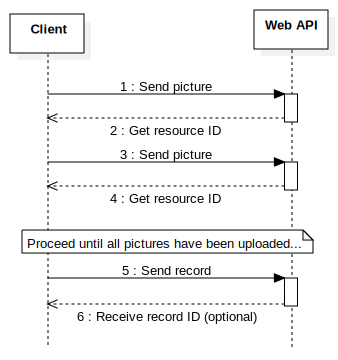
\includegraphics[scale=0.75]{server/working/SequenceDiagram-AddRecord.png}
            \caption{Sequence diagram: adding a record through the web API}
            \label{fig:addRecordSequenceDiagram}
        \end{figure}

        \begin{landscape}
            \begin{figure}
                \centering
                \includegraphics[scale=0.2]{server/ComponentDiagram.png}
                \caption{Web Api component Diagram}
                \label{fig:webAPIComponentDiagram}
            \end{figure}
        \end{landscape}

    \subsubsection{Significant data structures}

        The web API is going to make use of the Record and Specimen data structures, which will be exchanged between the server and its clients (the Android application and the website). They will be represented in a JSON format, which is readily available for use in PHP, JavaScript, and Android. Data types, where specified, are JSON data types. 

        The structure of a Record is as follows:
        \begin{itemize}
            \item Record : Object
            \begin{itemize}
                \item UserName : String
                \item UserPhone : String
                \item UserEmail : String
                \item LocationName : String 
                \item Timestamp : Number 
                \item LocationOS : String
                \item Specimens : Array of Specimen
            \end{itemize}
        \end{itemize}

        The structure of a Specimen is as follows:
        \begin{itemize}
            \item Specimen : Object
            \begin{itemize}
                \item SpeciesName : String
                \item LocationLatitude : Number
                \item LocationLongtitude : Number
                \item Abundance : Number
                \item Comment : String
                \item ScenePhoto : String (ID of a resource on the server)
                \item SpecimenPhoto : String (ID of a resource on the server)
            \end{itemize}
        \end{itemize}

        The web API is going to use a relational database as a data store.
        The database tables are as follows:

        \begin{itemize}
            \item Users
            \begin{itemize}
                \item UserId : INT auto-increment PK
                \item UserName : VARCHAR(20) not-null
                \item UserFullName : VARCHAR(50)
                \item UserPhone : VARCHAR(20)
                \item UserEmail : VARCHAR(50)
                \item UserPassword : BINARY(20)
            \end{itemize}
                
            \item Records
            \begin{itemize}
                \item RecordId : INT auto-increment PK
                \item UserId : INT not-null
                \item LocationName : VARCHAR(50)
                \item Timestamp : INT
                \item LocationOS : VARCHAR(10)
            \end{itemize}
                
            \item Resources
            \begin{itemize}
                \item ResourceId : INT auto-increment PK
            \end{itemize}

            \item Specimens
            \begin{itemize}
                \item SpecimenId : INT auto-increment PK
                \item RecordId : INT not-null
                \item SpeciesName : VARCHAR(255) not-null
                \item Latitude : FLOAT(10,6)
                \item Longitude : FLOAT(10,6)
                \item Abundance : INT
                \item Comment : TEXT
                \item ScenePhoto : INT
                \item SpecimenPhoto : INT   
            \end{itemize}
        \end{itemize}

    \begin{thebibliography}{9}
        \bibitem{refSpec} Project Plan Specification Standards :B. P. Tiddeman (2014-09-23) SE.QA.05b 1.2
    \end{thebibliography}

    \section{Document History}
        \begin{tabular}{l || p{8cm} | l | r}
            Version & Edit & Date & Persons \\ \hline 
            0.1 & Initial Version & November 5 2014 & nid21 \\ \hline
            0.2 & Updated with decomposition description & November 12 2014 & nid21 \\
            0.3 & Updated with Android interfaces & November 17 2014 & nid21 \\
            0.4 & Included web and server sections & November 27 2014 & nid21 \\
            0.5 & Document review & November 28 2014 & nid21 \\
            0.6 & More document reviewing and preparing for release & December 02 2014 & nid21 \\
        \end{tabular}

\end{document}
